%Sensor yang digunakan
%Aktuator ysng digunakan
%Microcontroller yang digunakan
%mini pc yang digunakan
%Interface yang digunakan

\begin{center}
    \section*{BAB 2 DASAR TEORI}
\end{center}

\setcounter{section}{2}
\setcounter{subsection}{0}


\subsection{Sensor}
    Sensor merupakan alat atau komponen elektronik yang memiliki kemampuan untuk mengidentifikasi perubahan dalam suatu kondisi lingkungan fisik\cite{sensor}.
    Sensor yang kami gunakan adalah LM35, LM35 sendiri adalah sensor suhu Analog yang akan menghasilkan tegangan voltase yang sebanding atau linear dengan suhu sekitarnya, sensor LM35 memiliki koefisien 10mV per Celcius dengan rentang kerja -55°C sampai 150°C. sensor LM35 juga memiliki akurasi yang tinggi dalam pembacaan data temperature, beberapa varian dari LM35 memiliki fitur untuk kompensasi suhu internal yang membuat sensor akan tetap akurat di berbagai kondisi. pada beberapa kasus, kalibrasi dalam sensor mungkin diperlukan untuk menjaga akkurasi dan beradaptasi pada lingkungan. lm35 memiliki 3 pinout, yang pertama ground sebagai referensi, Vin sebagai Vcc atau referensi kedua dan Vout sebagai pin output dari pengukuran suhu lm35. 

    \begin{figure}[H]
        \centering
        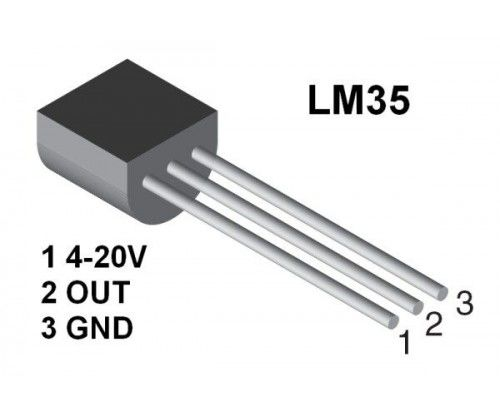
\includegraphics[width=8cm]{image/lm35-suhu.jpg}
        \caption{LM35}
        \captionsource{https://breakrow.com/mili-ampere/menggunakan-sensor-suhu-lm35-dengan-arduino}
        \label{fig:lm35}
    \end{figure}

\subsection{Aktuator}
    Peralatan mekanis untuk menggerakkan atau mengontrol sebuah sistem yang digunakan sebagai proses lanjutan dari keluaran suatu proses olah data yang dihasilkan dari sensor merupakan definisi dari aktuator\cite{aktuator}. Aktuator yang kami gunakan adalah lampu dan kipas. lampu diatur hidup mati menggunakan relay yang mendapatkan input dari mikrocontroller. lampu yang kami gunakan memiliki input voltase 220v ac. kipas juga diaturhidup mati menggunakan relay, kipas memiliki voltage converter karena kipas memiliki input voltase 12v Dc.
    \begin{figure}[H]
        \centering
        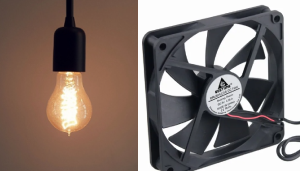
\includegraphics[width=10cm]{image/aktuator.png}
        \caption{Aktuator}
        \label{fig:aktuator}
    \end{figure}

\subsection{Arduino IDE}


Proses pemrograman Arduino dilakukan melalui Software Processing, yang dirancang untuk menulis program untuk Arduino. Processing sendiri merupakan gabungan dari bahasa C++ dan Java. Keunggulan Arduino terletak pada kemampuannya berupa kombinasi perangkat keras, bahasa pemrograman, dan Integrated Development Environment (IDE) yang canggih. IDE berperan penting dalam menulis program, mengkompilasi menjadi kode biner, dan mengunggahnya ke dalam memori mikrokontroler\cite{arduino-ide}.
\begin{figure}[H]
    \centering
    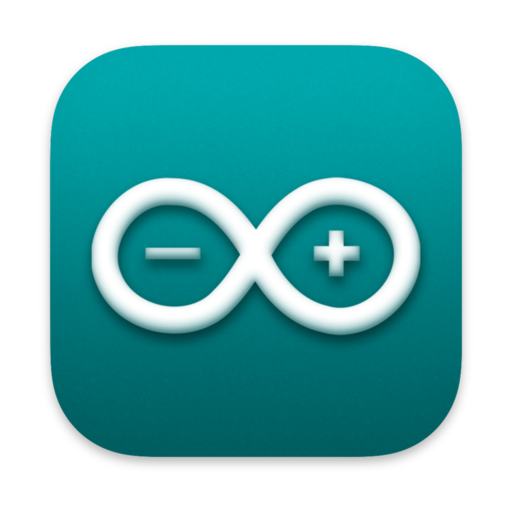
\includegraphics[width=3cm]{image/arduino-ide.png}
    \caption{Logo Arduino IDE}
    \captionsource{https://www.pngwing.com/en/free-png-adjvu/download}
    \label{fig:arduino-ide}
\end{figure}
Software IDE Arduino terdiri dari tiga bagian utama: editor program untuk menulis dan mengedit program dalam bahasa Processing, kompiler yang mengubah kode program menjadi kode biner yang dapat dipahami oleh mikrokontroler, dan uploader yang memasukkan kode biner ke dalam memori mikrokontroler. Selain itu, Arduino dapat diinstal pada berbagai sistem operasi seperti LINUX, Mac OS, dan Windows, menjadikannya alat pengembangan yang fleksibel dan dapat diakses oleh berbagai pengguna.\cite{arduino-ide}


\subsection{Mikrokontroller ESP-WROOM-32}

ESP32 adalah mikrokontroler System on Chip (SoC) terpadu yang dilengkapi dengan WiFi 802.11 b/g/n, Bluetooth versi 4.2, dan berbagai peripheral. Dengan fitur-fitur seperti GPIO (General Purpose Input Output), prosesor terintegrasi yang kuat, dan kemampuan penyimpanan internal, ESP32 dapat berfungsi sebagai pengganti mikrokontroler Arduino. Kelebihan lainnya termasuk dukungan untuk koneksi Wi-Fi langsung, memungkinkan pengguna untuk mengintegrasikan perangkat ini dengan mudah ke dalam proyek IoT atau aplikasi yang memerlukan konektivitas nirkabel. \cite{esp32}


ESP32 berperan ganda dalam proyek kami. Pertama, ia berfungsi sebagai publisher yang bertanggung jawab untuk menangkap data suhu melalui sensor LM35. Sensor ini memungkinkan pengukuran suhu yang akurat, dan ESP32 secara efisien mengirimkan informasi ini, memungkinkan pemantauan dan kontrol real-time.

\begin{figure}[H]
    \centering
    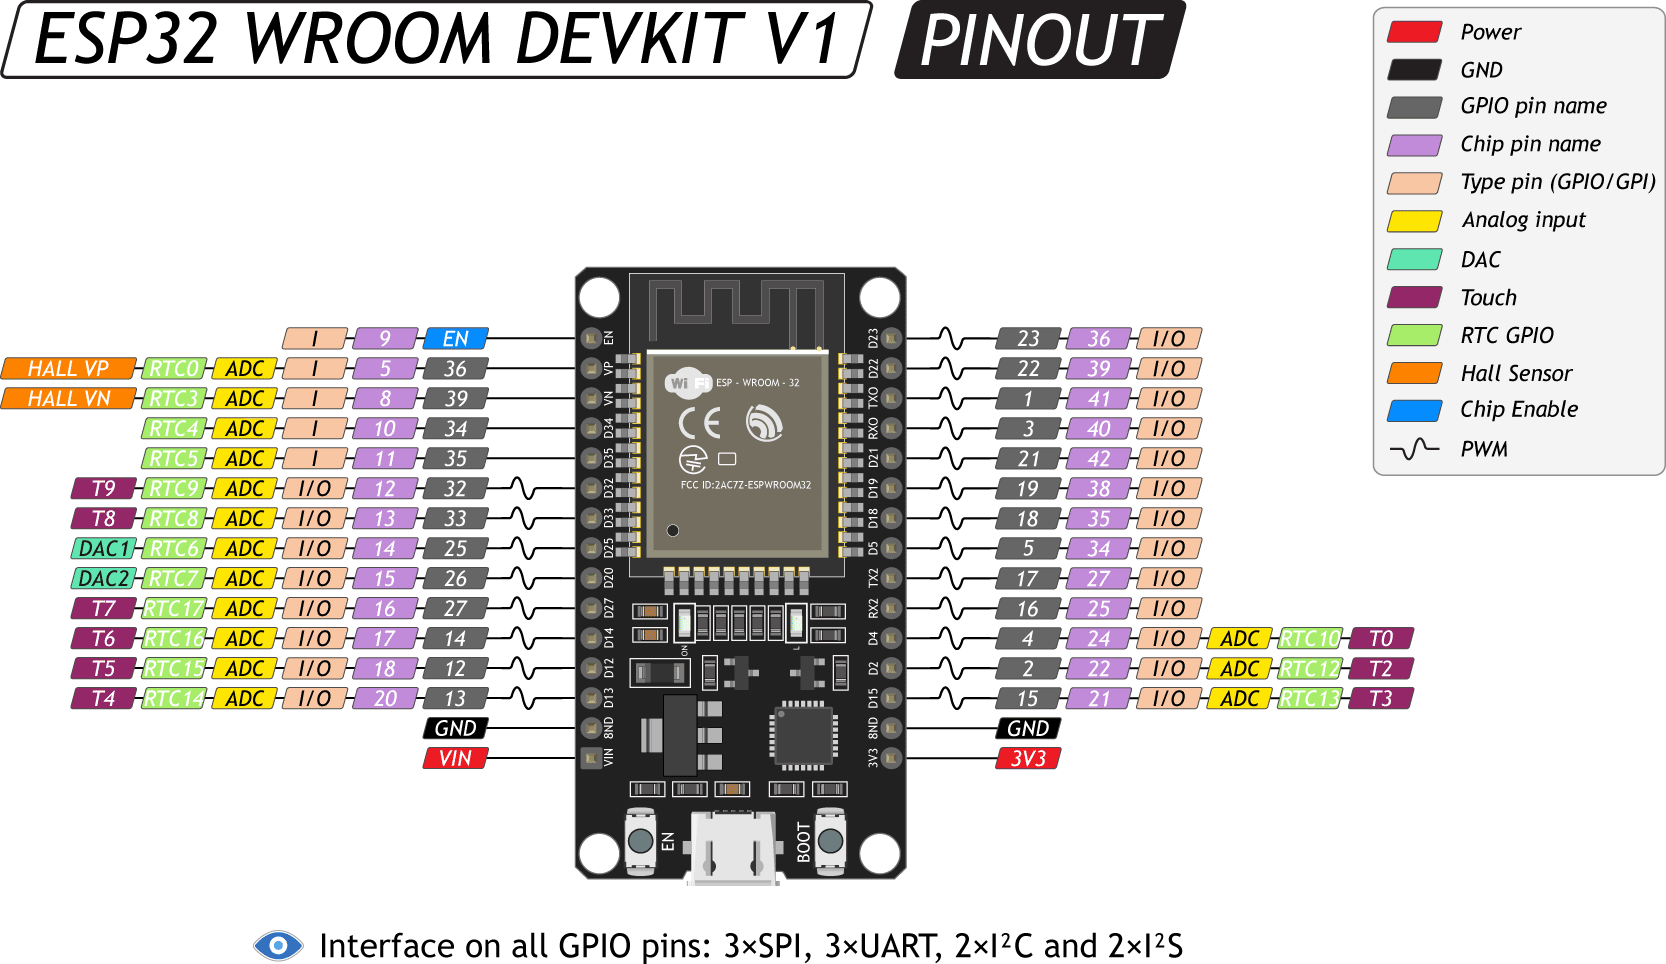
\includegraphics[width=10cm]{image/eps32pinout.png}
    \caption{ESP32 Pin Out}
    \captionsource{https://lastminuteengineers.com/esp32-pinout-reference/}
    \label{fig:esp32}
\end{figure}

Kedua, ESP32 mengemban peran sebagai pelanggan (subscriber), secara aktif terlibat dengan topik MQTT seperti "lampu" dan "kipas". Sebagai pelanggan, ESP32 merespons pesan yang masuk terkait dengan topik-topik ini, memungkinkannya untuk mengontrol perangkat yang terhubung. Fungsi dwi arah ini menunjukkan kemampuan ESP32 tidak hanya untuk mengumpulkan data sensor tetapi juga untuk berinteraksi dengan dan memengaruhi lingkungan sekitar berdasarkan pesan MQTT yang diterima.


\subsection{Raspberry Pi}


Raspberry Pi adalah sebuah komputer mini yang, dalam fungsinya, mirip dengan komputer umum namun dalam bentuk yang lebih kecil. Seperti board mikrokontroler pada umumnya, Raspberry Pi memiliki input dan output. Di antara seri produk Raspberry Pi, Raspberry Pi 4 model B menjadi pilihan unggul dengan peningkatan signifikan dalam hal kecepatan prosesor, multimedia, kinerja, memori, dan konektivitas jika dibandingkan dengan generasi sebelumnya. Yang menarik, meskipun memiliki kemampuan yang canggih, Raspberry Pi 4 model B tetap efisien dalam penggunaan daya listrik. Keunggulan lainnya terletak pada pin GPIO yang terprogram secara fleksibel, memungkinkan pengguna untuk mengumpulkan data atau mengendalikan modul sensor dengan menggunakan pin sebagai port serialnya \cite{raspi}.

Raspberry Pi memainkan peran kunci dalam proyek ini, digunakan untuk menginstal Mosquitto dan klien Mosquitto. Sebagai perangkat mini yang handal, Raspberry Pi memberikan platform yang ideal untuk menjalankan perangkat lunak MQTT broker seperti Mosquitto, memungkinkan komunikasi yang efisien antara perangkat yang terhubung dalam jaringan IoT kami.

\begin{figure}[H]
    \centering
    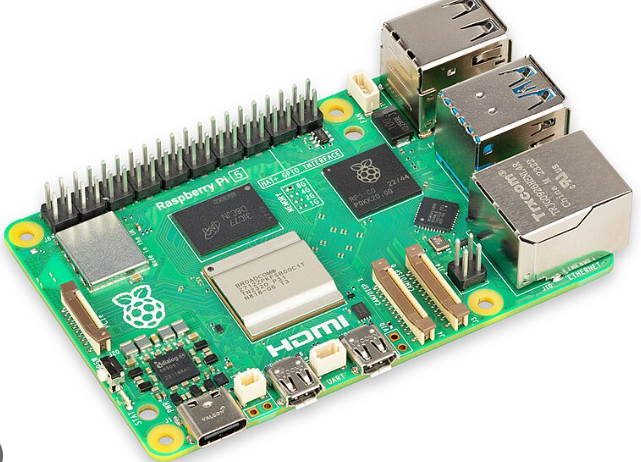
\includegraphics[width=8cm]{image/rasberry-pi.png}
    \caption{Raspberry Pi 4 Model B}
    \captionsource{https://www.yangcanggih.com/2019/06/24/raspberry-pi-4-model-b-performa-lebih-kencang-mendukung-video-4k-60fps/}
    \label{fig:raspi}
\end{figure}


Dengan menginstal Mosquitto di Raspberry Pi, kami membangun dasar komunikasi yang andal dan aman. Mosquitto berfungsi sebagai broker MQTT yang dapat diandalkan, menyediakan layanan yang mendukung pertukaran pesan antara perangkat dalam proyek kami. Penggunaan Raspberry Pi sebagai tuan rumah untuk Mosquitto dan klien Mosquitto memperkuat kontrol dan manajemen jaringan IoT kami, memberikan dasar yang kokoh untuk pengiriman dan penerimaan data yang efisien antara perangkat dalam ekosistem proyek kami.

\subsection{MQTT Protocol}
Dalam ekosistem Internet of Things (IoT), protokol MQTT menjadi protocol untuk mengatur komunikasi efisien antara perangkat.pada imlementasinya MQTT Protokol memiliki 3 object penting yaitu broker, publisher dan subcriber. Dalam implementasi ini, Raspberry Pi digunakan sebagai broker MQTT. yang memungkinkan komponen lingkungan IoT lainnya untuk berkomunikasi secara lancar.
\begin{figure}[H]
    \centering
    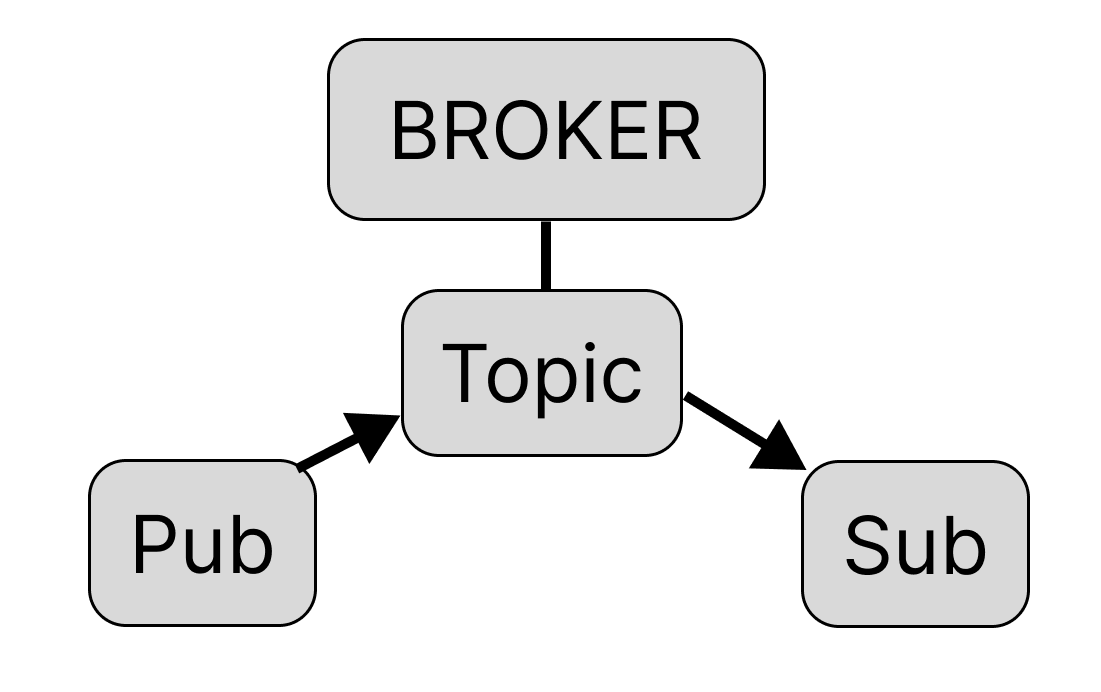
\includegraphics[width=6cm]{image/MQTT.png}
    \caption{MQTT}
    \label{fig:mqtt}
\end{figure}
ESP32, yang berperan ganda sebagai publisher dan subscriber, memainkan peran dalam mengumpulkan dan mendistribusikan data. Sebagai penerbit, ESP32 dapat mengirimkan data sensorik atau informasi lain ke broker MQTT di Raspberry Pi. Sebaliknya, sebagai pelanggan, ESP32 dapat mensubscribe untuk menerima informasi atau perintah tertentu dari topik yang relevan.
Selain itu, Node-RED Dashboard memberikan antarmuka pengguna yang interaktif untuk mengawasi dan mengontrol perangkat IoT. Dengan kemampuan Node-RED untuk berfungsi sebagai pelanggan dan penerbit MQTT, dashboard ini dapat menerima pembaruan dari komponen lain dan mengirimkan perintah kembali ke komponen pada lingkungan IoT. 

\subsection{Node-Red Dashboard}
Node-Red merupakan framework untuk iot yang sering digunakan. Node-red memiliki berbagai module yang bisa digunakan untuk menerima data dari MQTT, menerima data dari HTTP, menampilkan UI dashboard, dan berbagai fungsi lainnya. 

\begin{figure}[H]
    \centering
    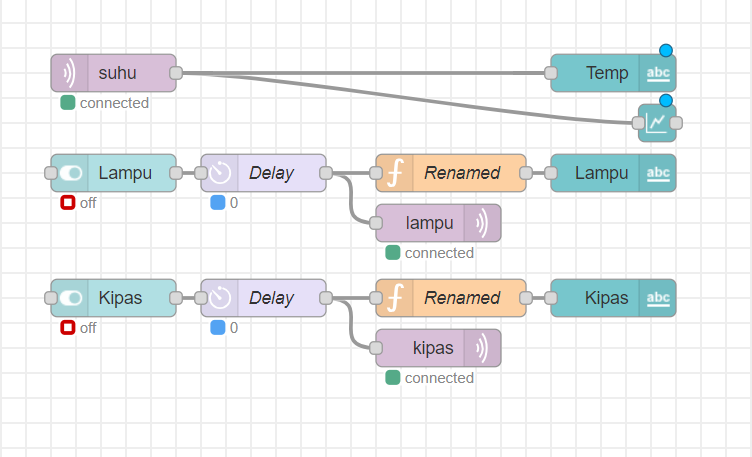
\includegraphics[width=13cm]{image/Node-red.png}
    \caption{Node-Red}
    \label{fig:node-red}
\end{figure}

pada implementasi kami, kami menerima data dari topic suhu mqtt pada rasberry pi broker, data ini akan di tampilkan dalam bentuk grafik. Dashboard dari node-red menyediakan kontrol untuk lampu dan kipas berupa switch untuk mengubah statenya secara manual. selain itu Dashboard dari node red juga menyediakan tampilan teks yang menampilkan suhu terakhir serta status aktif dari Lampu dan Kipas.